
\section{Experiments}
\subsection{Implementation Details}
\label{sec:implementation}

\subsubsection{\our}
Our \our\ model is built upon the Wan 2.2-TI2V-5B diffusion transformer~\citep{wang2025wan}, a 30-layer DiT with hidden dimension $d=3072$ and FFN dimension $14{,}336$. We extend its native single-branch RGB backbone into a unified tri-branch architecture for the synchronous synthesis of RGB, depth, and optical flow sequences. The depth and flow branches are initialized by duplicating the pre-trained components—patch embeddings, self-attention, normalization layers, and FFNs—leveraging the robust spatial-temporal priors of the video backbone. 

To ensure semantic alignment while minimizing overhead, we share the text cross-attention Key/Value projections across all three branches, as the linguistic task description provides a modality-agnostic semantic signal. We insert Joint Cross-Modal Attention (JA) modules every three transformer blocks across all 30 layers (at layers 0, 3, 6, \dots, 27), yielding 10 modules in total. For each branch $m$, the JA module queries the concatenated K/V pairs from the complementary modalities $j \neq m$:
\begin{equation}
    \hat{\bm{z}}_l^m = \bm{z}_l^m + \tanh(g_l^m) \cdot \operatorname{CrossBranchAttn}(\bm{Q}_l^m, \bm{K}_l^{\text{cross}}, \bm{V}_l^{\text{cross}}),
\end{equation}
where $g_l^m$ is a learnable scalar gate initialized to $1$. To ensure a smooth transition from independent branch training, we initialize the output projection to zero while keeping $g_l^m=1$. JA employs 3D RoPE and a frame-wise mask to restrict attention to tokens within the same temporal frame.

\paragraph{Phased Training Strategy.}
We adopt a three-stage curriculum to bridge modality distribution gaps. Tab.~\ref{tab:training_hparams} summarizes the stage-wise configuration. Each stage is initialized from the \emph{model-only} checkpoint of the previous stage (optimizer/scheduler reset) to ensure stability. We utilize the AdamW optimizer ($\beta_1{=}0.9, \beta_2{=}0.95$, weight decay $1{\times}10^{-4}$) with cosine scheduling and linear warm-up. We track an Exponential Moving Average (EMA, decay $0.9999$) with shadow weights on CPU for inference.

\paragraph{Stage 1: Modality Adaptation.}
Branches are trained independently under modality-specific flow-matching supervision to repurpose RGB priors for geometric and kinetic modeling without gradient interference. We use a learning rate of $2{\times}10^{-5}$ with $500$ warm-up steps and flow weight $\lambda_{\text{flow}}{=}0.5$.

\paragraph{Stage 2: Frozen-Backbone Joint Attention.}
We freeze the backbone and instantiate the 10 JA modules. To preserve established representations, we employ \textbf{zero-initialization} for the output projections of the JA modules. The learning rate is set to $5{\times}10^{-5}$ with $200$ warm-up steps. We apply Branch Dropout ($p_{\text{drop}}{=}0.2$) on $\{\text{depth}, \text{flow}\}$ to enhance cross-modal robustness.

\paragraph{Stage 3: Full-Parameter Joint SFT.}
We unfreeze the entire model for joint fine-tuning on the Rynn4DDataset 1.0.
We employ the learning rate as $1{\times}10^{-5}$ for all trainable parameters. Branch Dropout is reduced to $p_{\text{drop}}{=}0.1$.

\begin{table}[t]
\centering
\caption{Stage-wise training configuration. Effective batch size is per-GPU batch ($1$) $\times$ gradient accumulation (2-4) $\times$ $N_{\text{GPU}}$.}
\label{tab:training_hparams}
\setlength{\tabcolsep}{5pt}
\begin{tabular}{lccc}
\toprule
 & \textbf{Stage 1} & \textbf{Stage 2} & \textbf{Stage 3} \\
\midrule
\rowcolor{gray!10}Fusion mode & none & joint (frozen bb.) & joint (full SFT) \\
Trainable params & all branches & JA + mod.\ embed. & all parameters \\
\rowcolor{gray!10}Learning rate & $2{\times}10^{-5}$ & $5{\times}10^{-5}$ & $1{\times}10^{-5}$ \\
LR warm-up steps & $500$ & $200$ & $500$ \\
\rowcolor{gray!10}$\lambda_{\text{flow}}$ & $0.5$ & $1.0$ & $1.0$ \\
Branch Dropout & --- & $0.2$ & $0.1$ \\
\bottomrule
\end{tabular}
\end{table}

\paragraph{Resource and Optimization.}
All stages train at $81 \times 480 \times 640$ (yielding $T=21$ latent frames under the causal VAE's $4\times$ temporal compression, i.e., $T_{\text{latent}}=(T_{\text{pixel}}-1)/4+1$) with \texttt{bf16} mixed precision and gradient checkpointing. Stages 2 and 3 leverage DeepSpeed ZeRO-2 with optimizer offload to manage memory for additional JA parameters.









\begin{figure}[t]
  \centering
    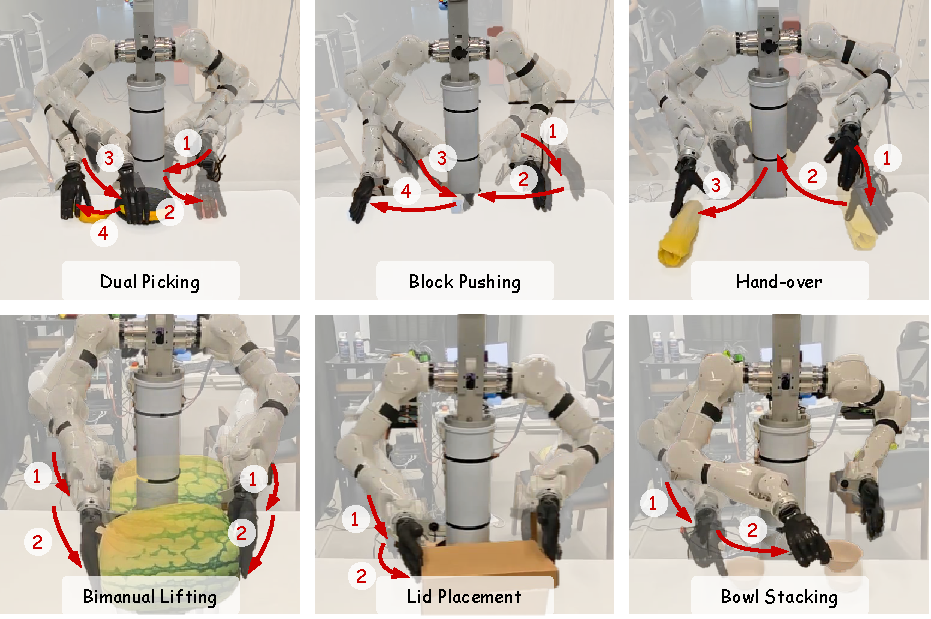
\includegraphics[width=\linewidth]{Fig/tasks.pdf}\\
    \caption{\textbf{Real-world Manipulation Benchmark.} We establish a comprehensive evaluation suite comprising six diverse tasks to assess the model's performance in open-world manipulation, providing a rigorous testbed for our 4D world model.}
  \label{fig:tasks}
\end{figure}

\subsubsection{\our-Policy}
We utilize \our\ as a frozen 4D vision encoder. The model operates at $480 \times 640$ resolution, producing $T=21$ latent frames (after VAE temporal compression with a ratio of 4). At each inference step, we perform single-step feature extraction at diffusion timestep $t=500$, capturing intermediate hidden states from block 15 of the transformer. By concatenating the 3072-dimensional features from the RGB, depth, and optical flow branches, we obtain a comprehensive 4D representation $F_p$.               

At each decision step, we take a single RGB observation frame as input. The condition frame is center-cropped to $480 \times 640$ and normalized to $[-1, 1]$. The extracted spatiotemporal features are reshaped and fed into Flow Former. This compresses the high-dimensional \our features into a fixed-size representation suitable for policy decoding.                        

We employ a flow matching policy head with 4-step Euler ODE sampling at inference time. Despite the multi-step sampling in the action space, the policy maintains high efficiency because the heavy 4D backbone features are only computed once. The policy predicts action chunks of length 10, where each action is 54-dimensional. During deployment, the model executes 10 actions open-loop before re-querying the visual backbone, yielding an effective control frequency of $\sim$9 Hz.

We train with AdamW optimizer using a learning rate of $1 \times 10^{-4}$, $\beta = (0.9, 0.9)$, and weight decay 0.05. We employ a tri-stage learning rate schedule: 2\% linear warmup, 8\% constant hold, and 90\% cosine decay to $10^{-6}\times$ the peak learning rate. The \our backbone is kept frozen throughout training; only the Flow Former and flow matching policy head are optimized. Training uses mixed precision with a batch size of 1 per GPU for 100 epochs. 


\subsection{Setups and Baselines}
\noindent 
\textbf{World model metrics.}
To evaluate the generative performance and physical fidelity of our world model, we conduct benchmarks on a held-out test set of 50 video sequences, randomly sampled from~\citep{wu2024robomind,liu2024rdt,jiang2025galaxea}. We assess the model across three axes: 
\begin{itemize}[labelsep=0.6em, leftmargin=1.2em,itemindent=0em]
    \item \textbf{(1) \textit{Visual Synthesis Quality}}: generative fidelity, following~\citep{zhou2025pai} (IQ, MS, SC, Subj.) and pixel-level alignment (PSNR, SSIM, LPIPS) with ground truth;
    
    \item \textbf{(2) \textit{Geometric Accuracy}}: evaluating structural integrity via depth estimation metrics (AbsRel, $\delta_1 < 1.25$); 
    
    \item \textbf{(3) \textit{Temporal Motion Consistency}}: measuring dynamic precision through optical flow error (AEPE). 
\end{itemize}
Detailed metric definitions are provided in Appendix~\ref{sec:metric}.




\noindent 
\textbf{Real-world task metric.} 
The primary evaluation metric is the Success Rate, defined as the percentage of successful task completions over 35 consecutive real-world trials. A trial is considered successful if the robot completes the task within 120 seconds.




\noindent 
\textbf{Hardware platform.} 
For real-world data collection and policy evaluation, we utilize the TIANJI M6 robot equipped with a WUJI HAND. A RealSense D435i camera is integrated to capture first-person view (FPV) images. Please refer to our Appendix.~\ref{sec:body} for more details.

\noindent 
\textbf{Robot tasks.}
\label{sec:tasks}
To demonstrate the generalization ability of our pipeline across diverse manipulation challenges, we evaluate our method on six distinct tasks that span varying levels of bimanual coordination, contact richness, and precision: 
\begin{itemize}[labelsep=0.6em, leftmargin=1.2em,itemindent=0em]
    \item \textbf{(1) \textit{Dual Picking}}: The robot uses its left arm to pick an apple and its right arm to pick a banana from a plate, sequentially placing both objects onto the tabletop.
    
    \item \textbf{(2) \textit{Block Pushing}}: A sequential pushing task where the left arm pushes a large block from the left zone to the center, after which the right arm takes over to push it to the designated right target zone.

    \item \textbf{(3) \textit{Hand-over}}: An intra-robot transfer task where the left gripper picks up a cabbage and hands it over to the right gripper, which then completes the placement.
    
    \item \textbf{(4) \textit{Bimanual Lifting}}: A heavy-load coordination task where both arms must synchronously lift a watermelon plush from the table and accurately place it into a tray.
    
    \item \textbf{(5) \textit{Lid Placement}}: A precision-oriented task requiring the robot to pick up a lid and accurately align it to cover a cardboard box.
    
    \item \textbf{(6) \textit{Bowl Stacking}}: There are two small bowls on the table; the task involves picking up one bowl and carefully stacking it on top of the other.
\end{itemize}





As shown in Fig.~\ref{fig:tasks}, these tasks collectively challenge the model's proficiency in dual-arm synergy, temporal sequencing, and long-horizon interaction.
Tab.~\ref{tab:dataset_stats} summarizes the per-task demonstration
budget: the full corpus is used to train \our, exposing it to a rich
diversity of physical interactions, while a fixed budget of 200 episodes
per task is allocated for training \our-Policy. 
For each task, we evaluate the model's generalization by applying significant randomization to the initial environment state. This includes varying the 6-DoF poses of task-relevant objects (\eg fruits) in terms of both workspace coordinates and axial rotations.

\begin{table}[t]
\centering
\caption{Statistics of the Real-World Dataset used for training.}
\label{tab:dataset_stats}
\begin{tabular}{lp{6cm}cc}
\hline
\textbf{Task Name} & \textbf{Description} & \textbf{RynnWorld-4D} & \textbf{RynnWorld-4D-Policy} \\ \hline
\rowcolor{gray!10}Dual Picking & Pick apple and banana from plate to table. & 500 & 200 \\
Block Pushing & Push block from left to center, then to the right. & 500 & 200 \\
\rowcolor{gray!10}Hand-over & Hand-over cabbage from left to right hand and place. & 300 & 200 \\
Bimanual Lifting & Lift a watermelon pillow and place it into a tray. & 500 & 200 \\
\rowcolor{gray!10}Lid Placement & Pick the lid and place it precisely on top of the box. & 300 & 200 \\ 
Bowl Stacking & Stack one bowl onto another. & 300 & 200 \\
\rowcolor{headerpurple!60} \textbf{Total} & & \textbf{2,400} & \textbf{1,200} \\ \hline
\end{tabular}
\end{table}








\begin{figure}
  \centering
    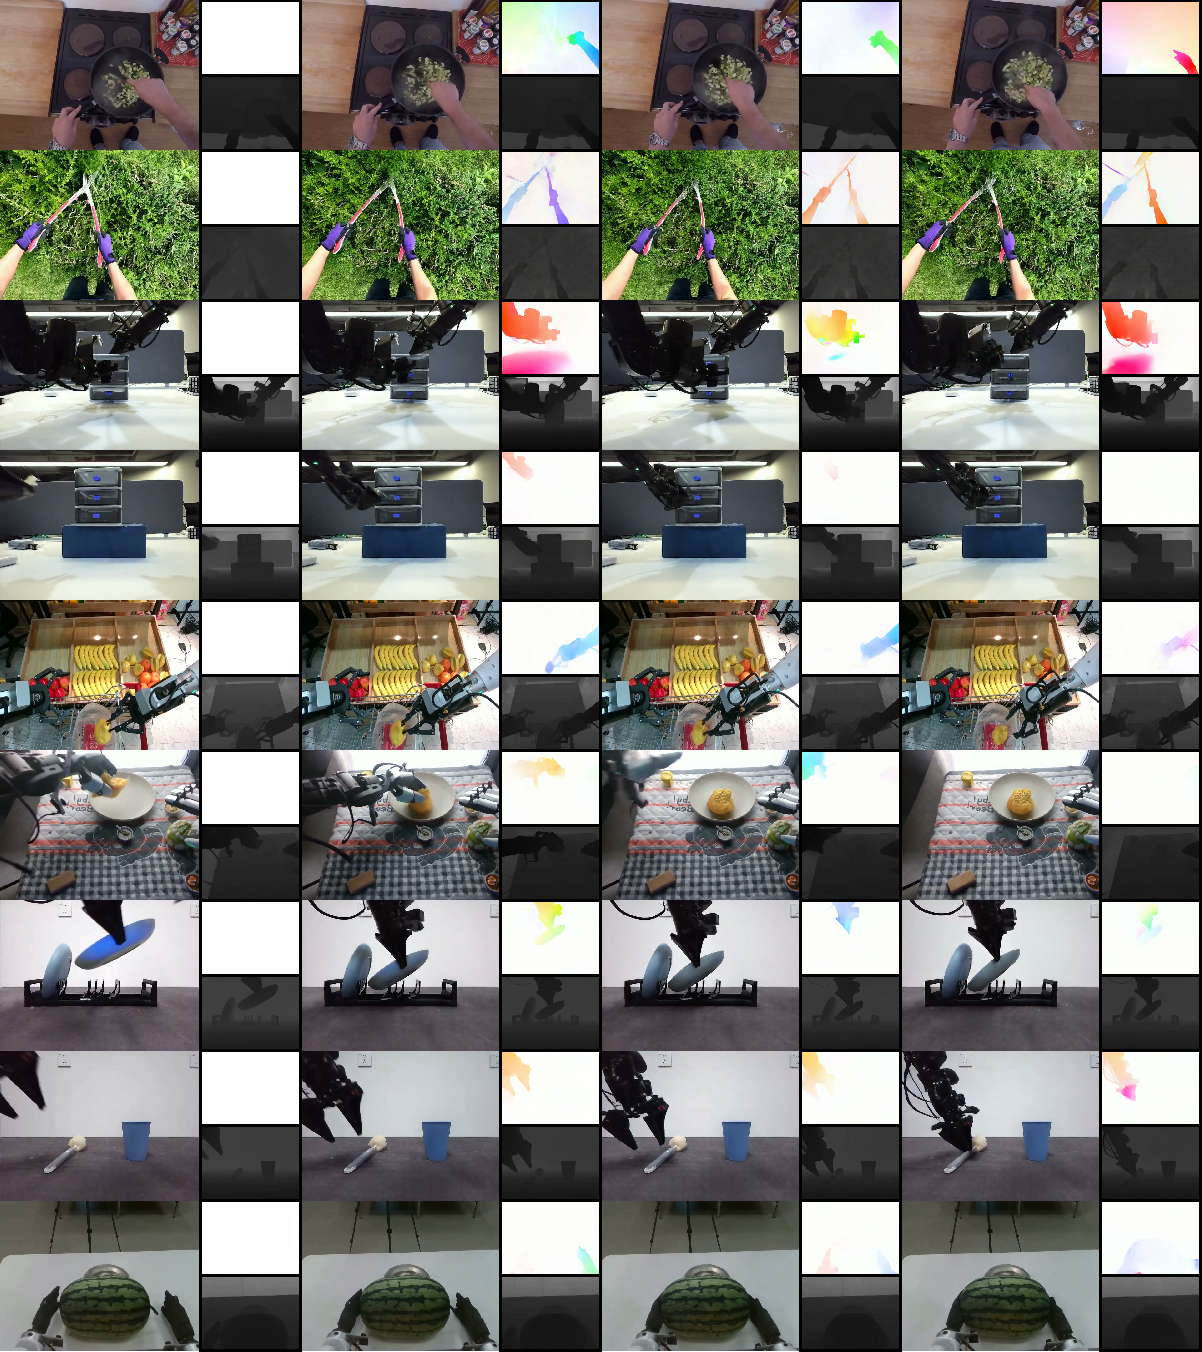
\includegraphics[width=\linewidth]{Fig/vis.pdf}\\
  \caption{\textbf{Qualitative results of \our.} Starting from a single RGB-D image and a text prompt, \our synchronously generates RGB video, depth maps, and optical flow, preserving sharp geometric structures and producing temporally consistent motion fields.}
  \label{fig:vis-flowoworld}
\end{figure}




\subsection{Results}
\noindent 
\textbf{4D World Modeling.}
As shown in Tab.~\ref{tab:exp}, compared to state-of-the-art video generation models such as Wan~\citep{wang2025wan} and CogVideoX~\citep{yang2024cogvideox}, \our maintains highly competitive visual quality (IQ) while significantly outperforming them in reconstruction fidelity. This indicates that while general video models excel at creative synthesis, our model is better at preserving the structural and textural integrity of the scene during evolution, benefiting from the mutual regularization between depth and flow branches. When compared to existing 4D world models, \our demonstrates a clear advantage in both spatial and temporal accuracy. In terms of geometry, our model achieves a $\delta_1$ of 0.610, nearly doubling the performance of 4DNeX~\citep{chen20254dnex} (0.327) and TesserAct~\citep{zhen2025learning} (0.279). Regarding motion, \our uniquely provides synchronized optical flow with a low AEPE of 0.170, whereas most baseline 4D models lack the capability to produce explicit motion fields. 

As visualized in Fig.~\ref{fig:vis-flowoworld}, the generated depth and flow maps are not only internally consistent but also precisely aligned with the RGB texture changes. This result validates our core hypothesis: jointly modeling RGB, depth, and flow within a single diffusion loop acts as a powerful physical regularizer. 



\begin{table*}[t]
 \centering
    \caption{\textbf{Quantitative evaluation of 4D world modeling quality.} Metrics span visual synthesis (RGB), geometric structure (Depth), and temporal dynamics (Optical Flow). N/A denotes that the baseline lacks the native capability to generate specific modalities.}
    \label{tab:exp}
    \small
    \setlength{\tabcolsep}{1.3pt} %
    \begin{tabular}{l ccc ccc c cc c}
    \toprule
    \multirow{2}{*}{\textbf{Method}} & \multicolumn{7}{c}{\textbf{RGB (Generation \& Fidelity)}} & \multicolumn{2}{c}{\textbf{Depth}} & \multicolumn{1}{c}{\textbf{Flow}} \\
    \cmidrule(lr){2-8} \cmidrule(lr){9-10} \cmidrule(lr){11-11}
    & IQ $\uparrow$ & MS $\uparrow$ & SC $\uparrow$ & Subj. $\uparrow$ & SSIM $\uparrow$ & PSNR $\uparrow$ & LPIPS $\downarrow$ & AbsRel $\downarrow$ & $\delta_1 \uparrow$ & AEPE $\downarrow$  \\
    \midrule
    \multicolumn{11}{c}{\textit{Video Generation Models}} \\
    \rowcolor{gray!10} CogVideoX~\citep{yang2024cogvideox} & 0.604 & 0.976 & 0.866 & 0.917 & 0.534 & 12.17 & 0.577 & N/A & N/A & N/A \\
    Wan-2.2-TI2V-5B~\citep{wang2025wan} & 0.555 & 0.970 & 0.886 & 0.909 & 0.593 & 14.54 & 0.489 & N/A & N/A & N/A \\
    \rowcolor{gray!10} Wan-2.1-I2V-14B~\citep{wang2025wan} & \textbf{0.684} & 0.988 & 0.891 & 0.956 & 0.536 & 12.72 & 0.568  & N/A & N/A & N/A \\

    \midrule
    \multicolumn{11}{c}{\textit{4D World Models}} \\
    \rowcolor{gray!10} Free4D~\citep{liu2025free4d} & 0.354 & 0.993 & 0.787 & 0.848 & 0.492 & 12.40 & 0.597 & 0.804 & 0.179 & N/A \\
    TesserAct~\citep{zhen2025learning} & 0.608 & 0.992 & 0.904 & 0.956 & 0.693 & 16.91 & 0.335 & 0.699 & 0.279 & N/A \\
    \rowcolor{gray!10} 4DNeX~\citep{chen20254dnex} & 0.637 & 0.994 & 0.917 & 0.986 & 0.649 & 14.47 & 0.404 & 0.423 & 0.327 & N/A \\
    \rowcolor{headerpurple!60} \textbf{\our}  & 0.635 & \textbf{0.995} & \textbf{0.957} & \textbf{0.992} & \textbf{0.754} & \textbf{17.85} & \textbf{0.269} & \textbf{0.310} & \textbf{0.610} & \textbf{0.170} \\

    \midrule
    \multicolumn{11}{c}{\textit{Ablation Study}} \\
    \rowcolor{gray!10} Independent Branches  & 0.613 & 0.986 & 0.922 & 0.971 & 0.683 & 17.26 & 0.346 & 0.737 & 0.245 & 0.247 \\
    w/o MA & 0.621 & 0.992 & 0.952 & 0.975 & 0.699 & 17.85 & 0.303 & 0.507 & 0.479 & 0.231 \\
    \rowcolor{gray!10} w/o 4D Pre-training & 0.615 & 0.982 & 0.879 & 0.938 & 0.651 & 16.25 & 0.344 & 0.797 & 0.263 & 0.729 \\
    w/o RoPE in JA & 0.628 & 0.990 & 0.935 & 0.980 & 0.710 & 17.10 & 0.295 & 0.420 & 0.450 & 0.210 \\
    \rowcolor{gray!10} shared FFN & 0.618 & 0.985 & 0.902 & 0.965 & 0.695 & 16.50 & 0.320 & 0.580 & 0.380 & 0.280 \\

    \bottomrule    
    \end{tabular}
\end{table*}









\noindent 
\textbf{Policy Learning.}
Tab.~\ref{tab:real} summarizes the performance of \our-Policy across various robotic manipulation tasks, where it consistently outperforms state-of-the-art baselines including Diffusion Policy (DP)~\citep{chi2025diffusion} and foundation models like $\pi_0$~\citep{black2024pi_0} and $\pi_{0.5}$~\citep{intelligence2025pi_}.

Notably, in tasks requiring high spatial precision such as \textit{Lid Placement} and \textit{Bowl Stacking}, \our-Policy achieves success rates of 65.71\%, surpassing the next best baseline (DP) by 8.57\%. 
Even more striking is the \textit{Hand-over} task, a challenge involving dynamic object transfer where foundation models struggle. 
This performance gap stems from two fundamental limitations of current foundation models: first, their pre-training data is predominantly biased towards parallel-jaw grippers, lacking the inherent priors for the complex dexterous hand coordination. Second, in a hand-over scenario, 2D-based models struggle to reason about the relative 3D distance and potential self-occlusion between two high-DOF end-effectors.
Furthermore, while these 2D policies must implicitly recover complex transfer dynamics from appearance residuals in the RGB stream, \our-Policy benefits from explicit kinetic and geometric cues provided by the world model's internal 4D latents, proving that predictive 4D representations are essential for tasks requiring precise temporal and spatial coordination where pure generative 2D priors fall short.


\begin{table*}[t]
 \centering
    \caption{\textbf{Success rates (\%) on robotic manipulation tasks.} We compare \our-Policy against state-of-the-art policy learning baselines and foundation models across six challenging tasks.}
    \label{tab:real}
    \small
 \begin{tabular}{l *{6}{>{\centering\arraybackslash}m{1.4cm}}}
 \toprule
  \textbf{Method}
 & \textbf{Dual Picking}
 & \textbf{Block Pushing}
 & \textbf{Hand-over}
 & \textbf{Bimanual Lifting}
 & \textbf{Lid Placement} 
 & \textbf{Bowl Stacking} \\
 \midrule
 \rowcolor{gray!10} DP~\citep{chi2025diffusion} & 77.14 & 85.71 & 17.14 & 88.57 & 57.14 & 57.14 \\
 $\pi_0$~\citep{black2024pi_0} & 88.57 & 94.29 & 2.86 & 91.43 & 34.29 & 51.43 \\
 \rowcolor{gray!10} $\pi_{0.5}$~\citep{intelligence2025pi_} & \textbf{94.29} & \textbf{100.00} & 0.00 & 94.29 & 37.14 & 42.86 \\
 \rowcolor{headerpurple!60} \textbf{\our-Policy} & \textbf{94.29} & 97.14 & \textbf{28.57} & \textbf{97.14} & \textbf{65.71} & \textbf{65.71} \\
 
 \midrule[\heavyrulewidth]
 \multicolumn{7}{c}{\textit{Ablation Study}} \\
 \rowcolor{gray!10} w/o \our  & 71.43 & 88.57 & 11.43 & 85.71 & 51.43 & 60.00 \\
 RGB  & 77.14 & 91.43 & 14.29 & 91.43 & 57.14 & 60.00 \\
 \rowcolor{gray!10} RGB + Depth  & 91.43 & 91.43 & 28.57 & 97.14 & 60.00 & 62.86 \\
 RGB + Optical Flow & 85.71 & 88.57 & 20.00 & 88.57 & 54.29 & 62.86 \\
 \bottomrule
 \end{tabular}
\end{table*}




\subsection{Ablation Study}
We conduct extensive ablation studies to validate our architectural design and training strategies.

\noindent 
\textbf{Effectiveness of Tri-branch Fusion.}
To verify the necessity of synchronized generation, we compare \our with the \textbf{Independent Branches} baseline, where three diffusion branches are trained separately. As shown in Tab.~\ref{tab:exp}, while independent branches can generate individual modalities, they suffer from significant performance degradation in depth (0.737 vs. 0.310 AbsRel) and flow (0.247 vs. 0.170 AEPE). This confirms that our mutual feature interaction mechanism is crucial for enforcing cross-modal consistency and physical fidelity in 4D sequences.


\noindent 
\textbf{Necessity of Modality Adaptation.}
The comparison between the full model and the \textbf{w/o MA} baseline (which skips the initial modality-specific adaptation and proceeds directly to joint tri-branch training) highlights the efficacy of our phased training strategy. Without this first stage, the depth and flow branches struggle to bridge the gap between their inherited RGB priors and their specific modality distributions (Tab.~\ref{tab:exp}). This leads to a substantial drop in geometric accuracy ($\delta_1$ decreases from 0.610 to 0.479) and compromised motion precision, proving that modality-specific adaptation is a prerequisite for effective multi-modal fusion.


\noindent 
\textbf{Significance of Large-scale 4D Pre-training.}
We evaluate the necessity of Rynn4DDataset 1.0 by comparing our full model with the \textbf{w/o 4D Pre-training} variant, which is trained exclusively on a limited set of task-specific robotic manipulation data. Omitting the large-scale pre-training on Rynn4DDataset 1.0 leads to a severe performance collapse across all dimensions, with the AEPE surging from 0.170 to 0.729 (Tab.~\ref{tab:exp}). These results underscore that task-specific data alone lacks the diversity required to master complex spatio-temporal dynamics.


\noindent
\textbf{Effectiveness of Predictive Latents.}
To verify the importance of the \our latent space, we compare our model against a baseline that replaces the predictive encoder with a standard ResNet-18~\citep{he2016deep} image encoder (\textbf{w/o \our} in Tab.~\ref{tab:real}). The significant performance drop across all tasks—most notably in \textit{Dual Picking} where success falls from 94.29\% to 71.43\%—highlights that static 2D features are insufficient for complex tasks. This confirms that the temporal and spatial dynamics captured in \our's predictive representations are crucial for robust policy learning.

\noindent
\textbf{Impact of 4D Modalities.}
We further analyze the individual contribution of each modality (Tab.~\ref{tab:real}). Using only RGB latents (\textbf{RGB}) yields sub-optimal success rates as the policy lacks explicit structural grounding. Integrating depth (\textbf{RGB + Depth}) provides significant gains in tasks requiring spatial precision, such as \textit{Hand-over} and \textit{Bimanual Lifting}. Meanwhile, adding optical flow (\textbf{RGB + Optical Flow}) enhances motion-sensitive tasks. The full \our-Policy, combining all three, achieves the best performance, confirming that the synergy of visual context, spatial geometry, and kinetic dynamics is essential for robust robotic manipulation.

\noindent 
\textbf{Role of 3D RoPE in Joint Attention.}
We disable the 3D Rotary Positional Embedding (RoPE) inside the Joint Cross-Modal Attention modules (\textbf{w/o RoPE in JA} in Tab.~\ref{tab:exp}) to decouple spatial coordinates from cross-modal interactions. Although intra-modal self-attention preserves local spatial structure, removing the shared positional bias in the cross-branch pathway disrupts the geometric correspondence between modality-specific features at identical $(u,v)$ coordinates. This misalignment manifests as a significant decay in reconstruction fidelity, with $\delta_1$ dropping from 0.610 to 0.450 and AEPE rising from 0.170 to 0.210. These results highlight that 3D RoPE serves as a critical alignment bridge, enabling the JA modules to achieve spatially-aware feature fusion at the pixel level rather than mere global semantic averaging.

\noindent 
\textbf{Per-branch FFN vs.\ Shared FFN.}
By default, our architecture employs independent feed-forward networks (FFNs) for each branch, initialized from the pre-trained RGB backbone to preserve specialized representation manifolds. Replacing these with a single FFN shared across all modalities (\textbf{Shared FFN} in Tab.~\ref{tab:exp}) leads to a systemic performance collapse. This suggests that the latent spaces of RGB textures, depth manifolds, and motion fields are inherently heterogeneous; forcing them through a shared non-linear transformation induces catastrophic interference in feature representation. The resulting decline in geometric accuracy (AbsRel 0.580 / $\delta_1$ 0.380) and motion stability (AEPE 0.280) empirically validates that modality-specific FFNs are essential to mitigate cross-modal distribution shifts and maintain high-fidelity 4D generation. Although this shared variant reduces parameter overhead, the substantial drop in generative fidelity underscores the necessity of modality-specific capacity in 4D world modeling.

